\chapter[Sistema de Comunicación]{Sistema de Comunicación}
\label{cp:comm-system}

%%% =========================================================
%%% 1. ARQUITECTURA GENERAL
%%% =========================================================
\section{Arquitectura General}
\label{sec:arq-general}

\subsection{Modelo de Capas y Responsabilidades}
\label{subsec:modelo-capas}

El sistema de comunicación se organiza en tres capas funcionales con responsabilidades
estrictamente delimitadas y fronteras bien definidas mediante interfaces abstractas.
Esta segmentación permite modificar o reemplazar cualquiera de las capas sin impactar a las
demás, siempre que se respeten los contratos establecidos.

\begin{figure}[htbp]
    \centering
    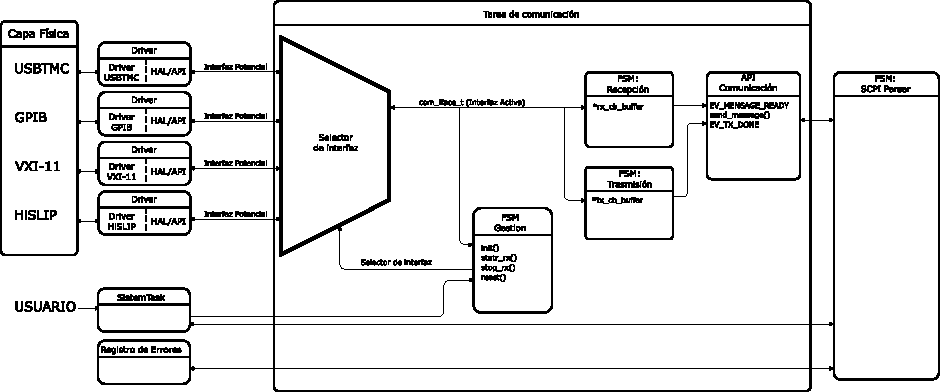
\includegraphics[width=0.85\textwidth]{Figuras/Schems/sitema-comunicacion.pdf}
    \caption{Modelo de capas del sistema de comunicación. Las flechas indican las
             dependencias funcionales y el sentido del flujo de datos.}
    \label{fig:capas-comunicacion}
\end{figure}

\paragraph{Capa de Driver (Interfaz de Transporte Físico)}

Es la capa más cercana al hardware. Su responsabilidad exclusiva es la gestión del periférico
de comunicación (UART, USBTMC, SPI, TCP/IP, etc.) y la traducción de eventos físicos a una
representación abstracta normalizada.

El driver expone sus servicios a través de la interfaz \texttt{comm\_iface\_t}, que constituye
un contrato cerrado. Toda implementación concreta debe cumplir con esta interfaz para ser
utilizable por las capas superiores. Esta abstracción oculta por completo las particularidades
del registro de periférico, las interrupciones, el DMA o los protocolos de enlace de bajo nivel.

La capa de driver:
\begin{itemize}
    \item Administra los recursos de hardware (registros, interrupciones, canales DMA).
    \item Produce eventos abstractos de interfaz (dato recibido, transmisión completada, error).
    \item Mantiene el estado operativo de la conexión física.
    \item No asigna buffers de aplicación ni realiza procesamiento de los datos transportados.
\end{itemize}

\paragraph{Capa de Middleware (Communication Task)}

Esta capa constituye el núcleo del subsistema de comunicación. Se implementa como una tarea
independiente (o un bucle dentro de un esquema cooperativo) y opera exclusivamente sobre la
interfaz abstracta proporcionada por el driver.

Sus responsabilidades comprenden:
\begin{itemize}
    \item La gestión global del ciclo de vida de la interfaz (inicialización, arranque,
          detención, recuperación ante fallos).
    \item La recepción de bytes desde el driver y la delimitación de mensajes completos de
          acuerdo con las reglas del protocolo de instrumentación (detección del terminador
          \texttt{LF} según IEEE~488.2).
    \item La transmisión de mensajes hacia el driver cuando la aplicación lo solicita.
    \item La publicación de eventos lógicos hacia la capa de aplicación:
          \texttt{EV\_MESSAGE\_READY} (mensaje disponible) y \texttt{EV\_TX\_DONE}
          (transmisión finalizada).
    \item La coordinación de las máquinas de estado de gestión, recepción y transmisión.
\end{itemize}

El middleware desconoce por completo el contenido semántico de los mensajes que transporta.
Un mensaje es, para esta capa, una secuencia de bytes delimitada por un terminador; no
realiza análisis sintáctico ni interpreta comandos.

\paragraph{Capa de Aplicación (Motor SCPI)}

Es la capa superior, consumidora de los servicios de comunicación. Recibe mensajes completos
desde el middleware y los procesa de acuerdo con la sintaxis y semántica del protocolo
SCPI (Standard Commands for Programmable Instruments).

Sus responsabilidades son:
\begin{itemize}
    \item El análisis sintáctico y semántico de los comandos recibidos.
    \item La ejecución de las acciones solicitadas (consulta de medidas, modificación de
          parámetros, etc.).
    \item La generación de respuestas conformes al estándar IEEE~488.2.
    \item La interacción con el resto del sistema del instrumento (control, medición,
          configuración).
\end{itemize}

El motor SCPI no accede directamente al hardware de comunicación ni a los buffers de
transporte. Para enviar una respuesta, invoca la función \texttt{send\_message()} expuesta
por el middleware.

\paragraph{Principio de Propiedad de Recursos}

Cada capa es propietaria exclusiva de los recursos que administra. Este principio evita
dependencias implícitas y condiciones de carrera:

\begin{itemize}
    \item Los buffers de transporte (recepción y transmisión) son propiedad de la
          \textit{Communication Task} y se inyectan al driver por referencia durante la
          inicialización. El driver opera sobre ellos pero no los posee.
    \item El contexto del periférico (registros de configuración, estado interno del driver)
          es privado de cada implementación concreta del driver y no es accesible desde fuera.
    \item Los buffers de comandos y respuestas SCPI pertenecen al motor SCPI y son
          independientes del transporte.
\end{itemize}

La tabla \ref{tab:propiedad-recursos} detalla la asignación de propiedad para cada recurso
compartido.

\begin{table}[htbp]
    \centering
    \caption{Propiedad de recursos en el sistema de comunicación.}
    \label{tab:propiedad-recursos}
    \begin{tabular}{lll}
        \toprule
        \textbf{Recurso} & \textbf{Propietario} & \textbf{Observación} \\
        \midrule
        Buffer RX de transporte & Communication Task & Asignado a la estructura \texttt{comm\_iface\_t} \\
        Buffer TX de transporte & Communication Task & Asignado a la estructura \texttt{comm\_iface\_t} \\
        Contexto del periférico  & Driver              & Privado de cada implementación \\
        Registro de eventos      & Driver              & Compartido ISR/Task mediante snapshot \\
        Estado de interfaz       & Driver              & Visible para capas superiores en modo lectura \\
        Buffers de comandos SCPI & Motor SCPI          & Independientes del transporte \\
        Buffers de respuesta SCPI& Motor SCPI          & Independientes del transporte \\
        \bottomrule
    \end{tabular}
\end{table}

\paragraph{Flujo de Información entre Capas}

La comunicación entre capas sigue un modelo orientado a eventos, sin llamadas bloqueantes.
El sentido del flujo es el siguiente:

\begin{description}
    \item[Recepción:] Medio físico $\rightarrow$ Driver $\rightarrow$ Eventos de interfaz
          $\rightarrow$ Communication Task $\rightarrow$ Mensaje completo $\rightarrow$
          Motor SCPI.
    \item[Transmisión:] Motor SCPI $\rightarrow$ Solicitud de transmisión $\rightarrow$
          Communication Task $\rightarrow$ Driver $\rightarrow$ Medio físico.
\end{description}

La capa de aplicación (Motor SCPI) se documenta en detalle en el capítulo siguiente. El
resto de este capítulo describe la arquitectura interna de las capas de Driver y Middleware,
así como las interfaces que las conectan.

\subsection{Propiedad de Recursos}
\label{subsec:propiedad-recursos}

La asignación explícita de la propiedad de cada recurso compartido es un principio
arquitectónico fundamental del sistema de comunicación. Establecer un propietario único para
cada estructura de datos, buffer o registro de estado persigue tres objetivos:

\begin{enumerate}
    \item \textbf{Eliminar la contención implícita:} cuando dos módulos pueden modificar
          un mismo recurso sin una mediación clara, aparecen condiciones de carrera y
          efectos laterales difíciles de depurar.
    \item \textbf{Permitir la verificación estática:} el propietario es responsable de
          asignar, liberar y garantizar la validez del recurso; los demás módulos lo
          utilizan bajo un contrato de acceso definido (lectura, escritura mediada, etc.).
    \item \textbf{Facilitar la portabilidad:} si cada recurso tiene un dueño bien
          identificado, reemplazar una capa (por ejemplo, cambiar el driver de USBTMC por
          uno de TCP/IP) no obliga a modificar la gestión de memoria de las demás capas.
\end{enumerate}

La tabla \ref{tab:propiedad-recursos} (presentada en la sección anterior) resume la
asignación de propiedad para los recursos principales. A continuación se detallan las
implicancias de cada caso.

\paragraph{Buffers de Transporte (RX y TX)}

Los buffers de recepción y transmisión a nivel de transporte son \textbf{propiedad exclusiva
de la \textit{Communication Task}}. Esto significa que:

\begin{itemize}
    \item La tarea de comunicación reserva estáticamente la memoria necesaria (por ejemplo,
          en su propio stack o en la sección \texttt{.bss} de su módulo objeto).
    \item Durante la inicialización, as referencias a estos buffers se asignan directamente en los campos \texttt{rx\_buffer} y \texttt{tx\_buffer} de la estructura \texttt{comm\_iface\_t} antes de invocar \texttt{init()}.
    \item El driver puede leer y escribir en ellos, pero \textbf{no es responsable de su
          ciclo de vida}. Si un driver necesita dimensionar los buffers, lo hace a través de
          parámetros de configuración, no asignándolos por sí mismo.
    \item Esta separación permite que, en un mismo hardware, dos interfaces distintas
          compartan la misma tarea de comunicación sin que el driver imponga un tamaño fijo
          de buffer.
\end{itemize}

\paragraph{Contexto del Periférico}

Cada implementación concreta del driver mantiene una estructura de contexto privada
(registros de configuración, estados internos, handles de sistema operativo, etc.). Este
contexto es \textbf{propiedad exclusiva del driver} y no es accesible desde la
\textit{Communication Task} ni desde la aplicación. Las capas superiores desconocen por
completo su contenido y solo interactúan con el driver a través de la interfaz abstracta
\texttt{comm\_iface\_t}.

Esta encapsulación garantiza que:

\begin{itemize}
    \item El middleware no pueda, por error, modificar un registro de periférico sin pasar
          por la API.
    \item Se pueda implementar un driver simulado (\textit{mock}) para pruebas unitarias
          del middleware, reemplazando completamente el contexto real sin que la tarea de
          comunicación lo advierta.
\end{itemize}

\paragraph{Registro de Eventos}

El registro de eventos es una estructura de mapa de bits (\textit{bitmask}) que el driver
actualiza de forma asíncrona (generalmente desde una ISR) y la \textit{Communication Task}
lee en cada ciclo. La \textbf{propiedad formal} reside en el driver, pero el acceso es
compartido:

\begin{itemize}
    \item Al inicio del siguiente ciclo de la \textit{Communication Task}, se captura
        atómicamente el registro de eventos del driver en una variable local
        (\textit{snapshot}) y se limpia el registro original. A partir de este momento,
        todas las FSM operan sobre la copia local, cada una enmascarando los bits que le
        corresponden.
    \item La \textit{Communication Task} \textbf{lee} el registro de manera atómica
          (mecanismo de \textit{snapshot} descrito en la sección \ref{subsec:snapshot}) y
          luego lo limpia.
    \item Ninguna otra capa accede directamente a este registro, ni siquiera en modo
          lectura. La aplicación recibe eventos lógicos de más alto nivel a través de la
          API de comunicación (\texttt{EV\_MESSAGE\_READY}, \texttt{EV\_TX\_DONE}).
\end{itemize}

\paragraph{Estado de la Interfaz}

El estado operativo de la interfaz (\texttt{COMM\_STATE\_CONNECTED},
\texttt{COMM\_STATE\_RX\_ACTIVE}, etc.) es mantenido por el driver y \textbf{visible en modo
lectura} para la \textit{Communication Task}. La tarea de middleware puede consultar este
estado para tomar decisiones de control (por ejemplo, no intentar transmitir si la interfaz
no está conectada), pero no puede modificarlo directamente. La modificación del estado es
consecuencia de las operaciones invocadas a través de la API (\texttt{start\_rx()},
\texttt{stop\_rx()}) o de eventos de hardware detectados por el driver.

\paragraph{Buffers de Comandos y Respuestas SCPI}

Los buffers donde se almacenan los comandos recibidos (ya delimitados) y las respuestas
generadas por el instrumento son \textbf{propiedad exclusiva del Motor SCPI}. Esta decisión
es crítica para la independencia de la aplicación respecto al transporte:

\begin{itemize}
    \item El middleware entrega el mensaje completo a la capa de aplicación copiándolo en el
          buffer de comandos SCPI o pasando una referencia que la aplicación debe consumir
          antes del siguiente ciclo de la tarea.
    \item La aplicación formatea sus respuestas en sus propios buffers y luego invoca
          \texttt{send\_message()} para transferirlas al middleware.
    \item Si en el futuro se reemplaza el protocolo SCPI por otro (por ejemplo, Modbus),
          los buffers de la aplicación cambian, pero el middleware de comunicación permanece
          inalterado.
\end{itemize}

\paragraph{Principio de Inyección de Dependencias}

La separación de propiedad se complementa con un patrón de \textbf{inyección de
dependencias} en tiempo de inicialización. La \textit{Communication Task} no instancia
directamente un driver concreto, sino que recibe una referencia a una implementación de
\texttt{comm\_iface\_t} junto con los parámetros de configuración necesarios (incluyendo las
referencias a los buffers de transporte). Este mecanismo, detallado en la sección
\ref{subsec:driver-buffers}, es el que permite que el mismo código de middleware opere sobre
UART, USBTMC o TCP/IP sin modificaciones.

\subsection{Conceptos Fundamentales}
\label{subsec:conceptos-fundamentales}

Para garantizar una interpretación unívoca de la arquitectura, esta sección define los
términos que se emplean de manera recurrente en la documentación del sistema de
comunicación. Cada concepto está acotado al contexto de este subsistema; otros módulos del
firmware pueden utilizar definiciones complementarias.

\paragraph{Estado}

Un estado representa una condición operativa persistente de una interfaz de comunicación.
Describe una situación que se mantiene durante un intervalo de tiempo y que puede consultarse
en cualquier momento.

En el sistema de comunicación, los estados se implementan como una máscara de bits
(\texttt{comm\_iface\_state\_t}), lo que permite que múltiples condiciones coexistan
simultáneamente. Por ejemplo, una interfaz puede estar al mismo tiempo
\texttt{CONNECTED} y \texttt{RX\_ACTIVE}.

Los estados son modificados exclusivamente por el driver como resultado de operaciones
solicitadas a través de la API (\texttt{start\_rx()}, \texttt{stop\_rx()}) o de eventos de
hardware detectados internamente. Las capas superiores pueden leerlos, pero no alterarlos
directamente.

\paragraph{Evento}

Un evento es la representación de un suceso instantáneo y asincrónico, producido por el
hardware de comunicación o por el propio driver. A diferencia de los estados, un evento no
describe una condición permanente sino una notificación puntual que debe ser procesada por
las capas superiores.

Los eventos se codifican como una máscara de bits (\texttt{comm\_iface\_event\_t}) en la que
cada bit representa un tipo de suceso. Esta representación permite:

\begin{itemize}
    \item La coexistencia de múltiples eventos simultáneos.
    \item El filtrado eficiente mediante operaciones de enmascaramiento binario.
    \item La transferencia atómica del registro completo (mecanismo de \textit{snapshot})
          entre el contexto de interrupción y el de tarea.
\end{itemize}

Ejemplos típicos de eventos son la disponibilidad de nuevos datos en el buffer de recepción,
la finalización de una transmisión o la detección de una condición de error de hardware.

\paragraph{Error}

Un error es una condición anómala detectada durante la operación de la interfaz de
comunicación. Los errores pueden originarse en el medio físico (errores de paridad, de
encuadre, desbordamiento del buffer de hardware), en la capa de transporte (timeout de
transmisión, fallo de bus) o en la propia implementación del driver (error interno).

La ocurrencia de un error se notifica mediante los eventos específicos definidos en
\texttt{comm\_iface\_event\_t} (\texttt{IFACE\_EVENT\_RX\_ERROR\_OVERFLOW},
\texttt{IFACE\_EVENT\_TX\_ERROR\_TIMEOUT}, etc.). Adicionalmente, un error crítico puede
provocar la activación del estado persistente \texttt{COMM\_STATE\_ERROR}, lo que indica a
las capas superiores que la interfaz no se encuentra en condición operativa normal.

Es importante distinguir entre el código de error retornado por algunas funciones de la API
(como \texttt{init()} o \texttt{reset()}) y los eventos de error asincrónicos. Los primeros
informan del resultado de una operación solicitada; los segundos notifican condiciones
sobrevenidas fuera del flujo de llamadas.

\paragraph{Operación}

Una operación es una acción explícita solicitada por una capa superior a través de la API de
la interfaz de comunicación. Constituye el mecanismo de control de que disponen la
\textit{Communication Task} y, de forma mediada, la aplicación, para gobernar el
comportamiento del driver sin exponer los detalles de implementación del periférico.

Las operaciones se corresponden con los \textit{callbacks} definidos en la estructura
\texttt{comm\_iface\_t}:

\begin{itemize}
    \item \textbf{Ciclo de vida:} \texttt{init()}, \texttt{deinit()}, \texttt{reset()}.
    \item \textbf{Control de flujo:} \texttt{start\_rx()}, \texttt{stop\_rx()},
          \texttt{start\_tx()}.
    \item \textbf{Acceso a datos:} \texttt{get\_char\_rx()}, \texttt{put\_char\_tx()}.
    \item \textbf{Gestión de eventos:} \texttt{set\_event()}, \texttt{get\_event()}.
    \item \textbf{Protección concurrente:} \texttt{protect\_rx()}, \texttt{unprotect\_rx()},
          \texttt{protect\_tx()}, \texttt{unprotect\_tx()}.
\end{itemize}

Todas las operaciones están diseñadas para ser no bloqueantes, en coherencia con el modelo
de ejecución cooperativa de la \textit{Communication Task}.

\paragraph{Contexto}

El contexto es una estructura de datos privada asociada a una instancia concreta de interfaz
de comunicación. En la implementación, la estructura \texttt{comm\_iface\_t} incluye un campo
\texttt{void *context} que cada driver utiliza para almacenar la información que necesita:
registros de configuración del periférico, handles del sistema operativo, punteros a buffers
internos, etc.

Ni la \textit{Communication Task} ni la capa de aplicación acceden al contenido del contexto;
solo lo pasan como argumento en cada invocación a los \textit{callbacks} del driver. Esta
opacidad garantiza la independencia de las capas superiores respecto de los detalles de
implementación del hardware.

\paragraph{Propietario}

El propietario de un recurso es el componente del sistema responsable de:

\begin{itemize}
    \item Reservar la memoria o el handle que lo representa.
    \item Garantizar su validez durante el tiempo de uso.
    \item Liberarlo cuando ya no es necesario.
\end{itemize}

La asignación de propiedad está explícitamente documentada en la tabla
\ref{tab:propiedad-recursos}. Los componentes que no son propietarios de un recurso pueden
utilizarlo únicamente bajo las condiciones establecidas por el contrato de acceso (por
ejemplo, el driver escribe en los buffers de transporte inyectados por la
\textit{Communication Task}, pero no es responsable de su asignación ni de su liberación).

\paragraph{Mensaje}

En el contexto del sistema de comunicación, un mensaje es la unidad de información que se
transfiere entre la \textit{Communication Task} y la capa de aplicación. Se define como una
secuencia contigua de bytes, delimitada por un carácter de fin de mensaje (el terminador
\texttt{LF}, \texttt{0x0A}, conforme a IEEE~488.2), y despojada de cualquier carácter de
control de transporte (como \texttt{CR}, \texttt{0x0D}).

La delimitación del mensaje es responsabilidad de la máquina de estados de recepción del
middleware. Una vez ensamblado el mensaje completo, se notifica a la aplicación mediante el
evento lógico \texttt{EV\_MESSAGE\_READY}. La aplicación puede entonces consumir el mensaje
desde el buffer de recepción de la \textit{Communication Task} (o copiarlo a sus buffers
propios) y proceder a su análisis sintáctico.

Análogamente, cuando la aplicación desea transmitir información, compone un mensaje en sus
buffers de respuesta y solicita el envío invocando \texttt{send\_message()}, lo que activa la
máquina de estados de transmisión del middleware.

Esta definición desacopla completamente el transporte del contenido: el middleware no
distingue entre un comando SCPI, una consulta de estado o cualquier otra carga útil; opera
exclusivamente con mensajes como secuencias de bytes delimitadas.

\subsection{Flujo de Comunicación}
\label{subsec:flujo-comunicacion}

El modelo de interacción entre capas es puramente asíncrono y orientado a eventos. No
existen llamadas bloqueantes ni dependencias cíclicas entre la \textit{Communication Task}
y la capa de aplicación. La secuencia de operaciones se describe a continuación para los
dos escenarios fundamentales: recepción de un mensaje y transmisión de una respuesta.

\paragraph{Flujo de Recepción}

\begin{enumerate}
    \item El medio físico entrega datos al periférico. La ISR del driver o el DMA
          transfieren los bytes al buffer de recepción inyectado (buffer circular o
          estructura de doble buffer, según la estrategia del driver).
    \item El driver activa en su registro de eventos el bit correspondiente a
          \texttt{IFACE\_EVENT\_RX\_DATA\_AVAILABLE}. Si se detecta una condición de error
          durante la recepción (overflow, framing, paridad), se activa el bit de error
          específico en lugar del de datos, o simultáneamente con él.
    \item En el siguiente ciclo de la \textit{Communication Task}, se ejecuta la captura
          atómica del registro de eventos (\textit{snapshot}) y se limpia el registro
          original.
    \item La FSM de Recepción consume los eventos del \textit{snapshot}. Si detecta
          \texttt{IFACE\_EVENT\_RX\_DATA\_AVAILABLE}, extrae uno a uno los bytes mediante
          \texttt{get\_char\_rx()} y los acumula en su espacio de trabajo.
    \item Cada byte es evaluado contra el terminador \texttt{LF} (\texttt{0x0A}). Los
          caracteres \texttt{CR} (\texttt{0x0D}) se descartan silenciosamente. Mientras no
          aparezca \texttt{LF}, la máquina permanece en el estado \texttt{RX\_GATHERING}.
    \item Al detectar el terminador, la FSM de Recepción considera el mensaje completo,
          retorna al estado \texttt{RX\_IDLE} y publica el evento lógico interno
          \texttt{EV\_MESSAGE\_READY}.
    \item La capa de aplicación (Motor SCPI), que es notificada de este evento en el mismo
          ciclo o en el siguiente según la implementación, toma el mensaje desde el buffer
          de recepción del middleware y procede a su análisis sintáctico.
\end{enumerate}

\paragraph{Flujo de Transmisión}

\begin{enumerate}
    \item La capa de aplicación, una vez generada una respuesta, invoca la función
          \texttt{send\_message()} provista por la API de la \textit{Communication Task},
          pasando la referencia al buffer de respuesta y su longitud.
    \item El middleware copia (o encola) los datos en su buffer de transmisión y activa
          internamente la señal \texttt{EV\_TX\_REQUEST}.
    \item La FSM de Transmisión, al evaluar este evento, transita al estado
          \texttt{TX\_BUSY} y comienza a transferir bytes al driver mediante llamadas
          sucesivas a \texttt{put\_char\_tx()}. Una vez cargado el bloque, invoca
          \texttt{start\_tx()} para iniciar la transmisión física.
    \item El driver maneja el envío (por interrupción o DMA). Al completarse, activa en su
          registro de eventos el bit \texttt{IFACE\_EVENT\_TX\_COMPLETE}.
    \item En el siguiente ciclo de la tarea de comunicación, la FSM de Transmisión captura
          este evento desde el \textit{snapshot}, retorna al estado \texttt{TX\_IDLE} y
          publica el evento lógico \texttt{EV\_TX\_DONE} hacia la aplicación.
    \item Si durante la transmisión se produce un error (timeout, fallo de bus), el driver
          activa el evento de error correspondiente. La FSM de Transmisión lo procesa,
          ejecuta \texttt{reset()} sobre el canal de transmisión y notifica el error a la
          aplicación a través de la API de comunicación.
\end{enumerate}

\paragraph{Sincronización y No Bloqueo}

Todo el ciclo de recepción y transmisión se ejecuta dentro del mismo hilo de la
\textit{Communication Task}, sin necesidad de semáforos ni colas adicionales. La
aplicación, si se ejecuta en el mismo contexto (esquema cooperativo), procesa los mensajes
de forma secuencial después de que la tarea de comunicación complete su ciclo. Si la
aplicación reside en una tarea separada, la transferencia se realiza mediante una cola de
mensajes —implementada como un buffer circular simple— que garantiza la entrega sin
bloqueo.

Este flujo será refinado con las máquinas de estado concretas en la sección de Middleware,
pero la descripción aquí presentada constituye el marco de referencia para todo el
subsistema.

%%% =========================================================
%%% 2. CAPA DE DRIVER (INTERFAZ DE TRANSPORTE FÍSICO)
%%% =========================================================
\section{Capa de Driver}
\label{sec:capa-driver}

La capa de driver constituye el punto de contacto entre el \textit{hardware} de comunicación
y el \textit{firmware} de nivel superior. Su misión es traducir las particularidades de cada
periférico físico a una representación abstracta y homogénea, de modo que el resto del
sistema pueda operar sin conocer los detalles de implementación del medio de transporte.

Esta sección describe el contrato que todo driver debe satisfacer —la interfaz abstracta
\texttt{comm\_iface\_t}—, los recursos que administra y las estrategias de sincronización
que emplea para operar de manera segura en un entorno con concurrencia.

\subsection{Interfaz Abstracta \texttt{comm\_iface\_t}}
\label{subsec:comm-iface}

La interfaz \texttt{comm\_iface\_t} es una estructura de punteros a función y campos de
datos que define el contrato vinculante para cualquier implementación de driver de
comunicación. Está diseñada para ser completamente agnóstica respecto del periférico
subyacente: UART, USBTMC, TCP/IP o cualquier otro medio pueden ser encapsulados detrás de
esta misma interfaz.

La estructura, definida en el código como \texttt{comm\_iface\_t}, contiene los siguientes
grupos funcionales:

\begin{itemize}
    \item \textbf{Identificación:} un campo \texttt{id} (\texttt{comm\_iface\_id\_t}) que
          identifica unívocamente la interfaz (USART, TCP, USBTMC) y un campo \texttt{name}
          legible para diagnóstico.
    \item \textbf{Contexto privado:} un puntero opaco \texttt{void *context} que cada
          implementación concreta utiliza para almacenar sus datos internos (registros del
          periférico, handles, buffers auxiliares). Ni la \textit{Communication Task} ni la
          aplicación acceden a este campo; simplemente lo reenvían en cada invocación a los
          \textit{callbacks}.
    \item \textbf{Estado y eventos:} los campos \texttt{state} (\texttt{comm\_iface\_state\_t})
          y \texttt{event} (\texttt{comm\_iface\_event\_t}) mantienen, respectivamente, la
          condición operativa actual de la interfaz y el registro de eventos pendientes de
          procesar.
    \item \textbf{Buffers de transporte inyectados:} punteros \texttt{rx\_buffer} y
          \texttt{tx\_buffer} a sendos \textit{buffers circulares}. Estos buffers son
          propiedad de la \textit{Communication Task} y se asignan a la estructura antes de
          invocar \texttt{init()}. El driver los utiliza como espacio de trabajo para la
          transferencia de datos, pero no es responsable de su asignación ni de su
          liberación.
    \item \textbf{Callbacks de ciclo de vida:} \texttt{init()}, \texttt{deinit()} y
          \texttt{reset()}. Gestionan la inicialización, desinicialización y reinicio del
          periférico. Retornan un código de error de tipo \texttt{comm\_error\_t} para
          informar del resultado de la operación.
    \item \textbf{Callbacks de control de flujo:} \texttt{start\_rx()}, \texttt{stop\_rx()}
          y \texttt{start\_tx()}. Activan y desactivan la recepción, e inician la
          transmisión de un bloque de datos previamente cargado.
    \item \textbf{Callbacks de acceso a datos:} \texttt{get\_char\_rx()} y
          \texttt{put\_char\_tx()}. Son las primitivas de lectura y escritura de bytes
          individuales sobre los buffers de transporte. Ambas son no bloqueantes: retornan
          un valor booleano que indica si la operación tuvo éxito.
    \item \textbf{Callbacks de gestión de eventos:} \texttt{set\_event()} y
          \texttt{get\_event()}. Permiten escribir y leer el registro de eventos de la
          interfaz. \texttt{get\_event()} es utilizado por la \textit{Communication Task}
          para obtener el \textit{snapshot} atómico al inicio de cada ciclo.
    \item \textbf{Callbacks de protección concurrente:} \texttt{protect\_rx()},
          \texttt{unprotect\_rx()}, \texttt{protect\_tx()} y \texttt{unprotect\_tx()}.
          Proveen mecanismos de exclusión mutua para el acceso a los buffers de recepción y
          transmisión desde contextos concurrentes (ISR y tarea). La implementación concreta
          de estos \textit{callbacks} depende del hardware y del sistema operativo
          subyacente; las capas superiores los invocan sin conocer su estrategia interna.
\end{itemize}

La figura \ref{fig:comm-iface-estructura} muestra un diagrama esquemático de la estructura
\texttt{comm\_iface\_t} y su relación con los componentes que la utilizan.

\begin{figure}[htbp]
    \centering
    % Diagrama: comm_iface_t como bloque central, con entradas de la Communication Task
    % (rx_buffer, tx_buffer inyectados) y flechas hacia el driver concreto (init, get_char, etc.)
    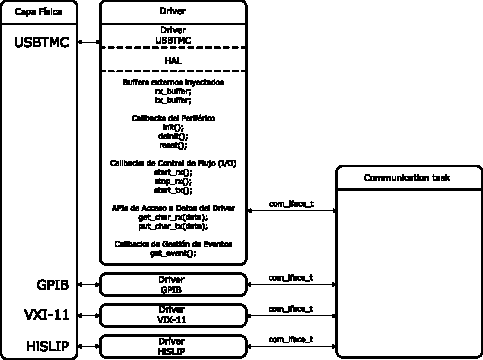
\includegraphics[width=0.7\textwidth]{Figuras/Schems/comm_iface_t.pdf}
    \caption{Estructura \texttt{comm\_iface\_t} y su interacción con la
             \textit{Communication Task} y el driver concreto.}
    \label{fig:comm-iface-estructura}
\end{figure}

La interfaz \texttt{comm\_iface\_t} es el único punto de acoplamiento entre el middleware
y el hardware de comunicaciones. Cualquier driver que implemente correctamente estos
\textit{callbacks} y respete la semántica de los campos de estado y eventos podrá ser
utilizado por la \textit{Communication Task} sin modificar una sola línea de su código.

   \subsection{Estados de la Interfaz}
   % - Máscara de estados (COMM_STATE_CONNECTED, RX_ACTIVE, TX_ACTIVE, ERROR).
   % - Coexistencia simultánea de estados.

   \subsection{Eventos de Comunicación y Error}
   % - Eventos de comunicación: IFACE_EVENT_INTERFACE_CONNECTED, DISCONNECTED, RX_DATA_AVAILABLE, TX_COMPLETE.
   % - Eventos de error: OVERFLOW, FRAMING, PARITY, TIMEOUT, BUS_FAULT, INTERNAL_ERROR.
   % - Relación con activación del estado COMM_STATE_ERROR.

   \subsection{APIs de Ciclo de Vida}
   % - init(), deinit(), reset(), start_rx(), stop_rx(), start_tx().
   % - Descripción de cada una y en qué fase se invocan.

   \subsection{APIs de Acceso a Datos}
   % - get_char_rx(), put_char_tx(), get_event(), set_event().
   % - Énfasis en que son no bloqueantes.

   \subsection{Protección de Acceso Concurrente}
   % - protect_rx() / unprotect_rx(), protect_tx() / unprotect_tx().
   % - Explicación de que aíslan a las capas superiores de la estrategia de sincronización concreta 
   %   (ISR vs. tarea).

   \subsection{Estrategias de Sincronización y Gestión de Buffers}
   \label{subsec:driver-buffers}
      \subsubsection{Inyección de Dependencias y Propiedad de Memoria}
      % - La Communication Task reserva los buffers y los pasa al driver en init().
      % - El driver solo actualiza índices y notifica eventos.

      \subsubsection{Buffer Circular Single-Producer-Single-Consumer (SPSC)}
      % - Para periféricos con DMA o interrupciones (ej. UART).
      % - ISR escribe en head, tarea lee hasta head capturado.
      % - Detección de overflow en ISR.

      \subsubsection{Estrategia de Doble Buffer (Even/Odd)}
      % - Para periféricos sin DMA generalizado.
      % - Swapping instantáneo de buffers; overflow si el buffer previo no fue procesado.

%%% =========================================================
%%% 3. CAPA DE MIDDLEWARE (COMMUNICATION TASK)
%%% =========================================================
\section{Capa de Middleware (Communication Task)}
\label{sec:middleware}

   \subsection{Modelo de Ejecución y Planificación}
   % - Hilo independiente o super-loop cooperativo.
   % - Evaluación no bloqueante de FSMs.
   % - Base de tiempo común (sys_tick) para timeouts.
   % - Determinismo al ejecutar todo en un único contexto.

   \subsection{Registro de Eventos y Captura Atómica (Snapshot)}
   \label{subsec:snapshot}
   % - El driver expone un registro de eventos en mapa de bits.
   % - Al inicio de cada ciclo: snapshot atómico (lectura + limpieza).
   % - Cada FSM aplica máscara binaria sobre el snapshot local.

   \subsection{Orden de Precedencia y Flujo de Control}
   % - Jerarquía: Gestión → RX → TX.
   % - Si hay error crítico, la FSM de Gestión interviene antes de procesar datos.
   % - El flujo del bucle: Snapshot → FSM Gestión → FSM RX → FSM TX → espera.

   \subsection{Máquinas de Estado de Transporte}
   \label{subsec:fsms-transporte}
      \subsubsection{FSM de Gestión de Interfaz}
      % - Supervisa el estado global: DOWN, READY, ACTIVE, ERROR.
      % - Tabla de transiciones original (adaptada para no incluir eventos SCPI).
      % - Acciones: init(), start_rx(), stop_rx(), deinit(), reset().

      \subsubsection{FSM de Recepción (RX)}
      % - Estados: RX_IDLE, RX_GATHERING.
      % - Transiciones basadas en IFACE_EVENT_RX_DATA_AVAILABLE y bytes leídos.
      % - Detección de LF para delimitar mensaje; descarte silencioso de CR.
      % - Al completar mensaje: publica EV_MESSAGE_READY (evento lógico interno).
      % - Manejo de errores de RX (overflow, framing, parity) → publica error y vuelve a IDLE.
      % - Tabla de transiciones adaptada.

      \subsubsection{FSM de Transmisión (TX)}
      % - Estados: TX_IDLE, TX_BUSY.
      % - Disparo por solicitud de la aplicación (EV_TX_REQUEST).
      % - Carga de datos vía put_char(), start_transmission().
      % - Al completar: publica EV_TX_DONE.
      % - Timeout de TX: reset_transmission() y error.

   \subsection{API de Servicios hacia la Capa de Aplicación}
   \label{subsec:api-aplicacion}
   % - Definición de los dos eventos lógicos que el middleware expone a la capa superior:
   %   · EV_MESSAGE_READY: buffer con mensaje completo (terminado en LF) listo para ser consumido.
   %   · EV_TX_DONE: confirmación de que la transmisión se completó exitosamente.
   % - Función send_message(const uint8_t *data, size_t len): la aplicación la llama para 
   %   encolar una respuesta en el buffer de TX del middleware y generar EV_TX_REQUEST.
   % - Se aclara que el buffer del mensaje de recepción pertenece a la Communication Task y 
   %   debe ser copiado/procesado antes del siguiente ciclo.

   \subsection{Adaptación a Protocolos de Instrumentación}
   % - Se describe cómo la FSM de RX se encarga de la delimitación según IEEE 488.2 (LF).
   % - El middleware no interpreta el contenido del mensaje.
   % - Mecanismo de "Query Interrupts": el driver traduce condiciones de hardware a eventos 
   %   abstractos; la FSM de Gestión los maneja sin invadir la capa de aplicación.
   % - Se deja explícito que el procesamiento sintáctico y semántico corresponde al Motor SCPI 
   %   (capítulo siguiente).

   \subsection{Selector de Medio de Transporte}
   % - Componente que asigna la interfaz física concreta al middleware en tiempo de inicialización.
   % - Opera sobre la abstracción comm_iface_t, permitiendo cambiar USBTMC, GPIB, TCP sin 
   %   modificar el middleware ni la aplicación.
El sistema de comunicación constituye una arquitectura en capas donde cada componente tiene una responsabilidad bien definida y posee explícitamente los recursos que administra.

\subsection{Propiedad de Recursos}

\begin{center}
\begin{tabular}{lll}
\toprule
\textbf{Recurso} & \textbf{Propietario} & \textbf{Observación} \\
\midrule
Buffer RX Transporte & Communication Task & Inyectado al driver durante el registro de interfaz \\
Buffer TX Transporte & Communication Task & Inyectado al driver durante el registro de interfaz \\
Contexto del Periférico & Driver & Privado de cada implementación \\
Registro de Eventos & Interfaz de Comunicación & Compartido ISR \\
                    &                           & Task mediante Snapshot \\
Estado de Interfaz & Interfaz de Comunicación & Visible para capas superiores en modo lectura \\
Buffers de Comandos SCPI & Motor SCPI & Independientes del transporte \\
Buffers de Respuesta SCPI & Motor SCPI & Independientes del transporte \\
\bottomrule
\end{tabular}
\end{center}

El driver no realiza asignación dinámica de memoria ni posee buffers propios de aplicación. Los buffers de transporte son propiedad exclusiva de la Communication Task y son inyectados mediante referencias durante la fase de inicialización de la interfaz.

\section{Interfaz de la Capa Física (Driver)}
\label{sec:interfaz-driver}

Cada interfaz física implementa un contrato estricto mediante una instancia de \texttt{comm\_iface\_t}. Esta estructura abstrae completamente las particularidades del hardware subyacente (UART, USBTMC, TCP/IP, etc.) y constituye el único mecanismo de interacción entre la \textit{Communication\_Task} y el medio de transporte.

La implementación concreta del driver es responsable exclusivamente de la gestión del transporte físico y de la traducción de eventos de hardware a eventos abstractos de interfaz.

\paragraph{Estados de Interfaz}

La condición operativa de una interfaz se representa mediante una máscara de estados (\textit{bitmask}):

\begin{itemize}
\item \texttt{COMM\_STATE\_CONNECTED}: Existe una conexión física o lógica válida.
\item \texttt{COMM\_STATE\_RX\_ACTIVE}: La interfaz posee datos pendientes de recepción o se encuentra recibiendo información.
\item \texttt{COMM\_STATE\_TX\_ACTIVE}: Existe una transmisión física en curso.
\item \texttt{COMM\_STATE\_ERROR}: Se detectó una condición de falla persistente en la interfaz.
\end{itemize}

Los estados representan condiciones persistentes y pueden coexistir simultáneamente.

\paragraph{Eventos de Comunicación}

Los eventos representan sucesos instantáneos producidos por el hardware o por el propio driver:

\begin{itemize}
\item \texttt{IFACE\_EVENT\_INTERFACE\_CONNECTED}
\item \texttt{IFACE\_EVENT\_INTERFACE\_DISCONNECTED}
\item \texttt{IFACE\_EVENT\_RX\_DATA\_AVAILABLE}
\item \texttt{IFACE\_EVENT\_TX\_COMPLETE}
\end{itemize}

\paragraph{Eventos de Error}

Las condiciones anómalas también se notifican mediante eventos:

\begin{itemize}
\item \texttt{IFACE\_EVENT\_RX\_ERROR\_OVERFLOW}
\item \texttt{IFACE\_EVENT\_RX\_ERROR\_FRAMING}
\item \texttt{IFACE\_EVENT\_RX\_ERROR\_PARITY}
\item \texttt{IFACE\_EVENT\_TX\_ERROR\_TIMEOUT}
\item \texttt{IFACE\_EVENT\_TX\_ERROR\_BUS\_FAULT}
\item \texttt{IFACE\_EVENT\_INTERNAL\_ERROR}
\end{itemize}

La ocurrencia de un evento de error puede provocar adicionalmente la activación del estado persistente \texttt{COMM\_STATE\_ERROR}.

\paragraph{APIs de Ciclo de Vida}

\begin{itemize}
\item \texttt{init()}
\item \texttt{deinit()}
\item \texttt{reset()}
\item \texttt{start\_rx()}
\item \texttt{stop\_rx()}
\item \texttt{start\_tx()}
\end{itemize}

\paragraph{APIs de Acceso a Datos}

\begin{itemize}
\item \texttt{get\_char\_rx()}
\item \texttt{put\_char\_tx()}
\item \texttt{get\_event()}
\item \texttt{set\_event()}
\end{itemize}

\paragraph{Protección de Acceso Concurrente}

La interfaz provee mecanismos de protección específicos de cada implementación para sincronizar el acceso concurrente entre ISR y contexto de tarea:

\begin{itemize}
\item \texttt{protect\_rx()}
\item \texttt{unprotect\_rx()}
\item \texttt{protect\_tx()}
\item \texttt{unprotect\_tx()}
\end{itemize}

Las capas superiores permanecen completamente desacopladas de la estrategia concreta utilizada por cada periférico.

\subsection{Responsabilidades por Componente}
\label{subsec:responsabilidades-componentes}

\subsubsection{Interfaz de Transporte}

La interfaz de comunicación es responsable de:

\begin{itemize}
\item Inicializar y configurar la implementación de comunicación asociada.
\item Configurar y administrar los recursos necesarios para la transferencia de datos.
\item Gestionar la recepción de información proveniente del medio de comunicación.
\item Iniciar transmisiones solicitadas por las capas superiores.
\item Detectar eventos relevantes producidos por la implementación subyacente.
\item Detectar y reportar errores de comunicación.
\item Publicar eventos hacia el subsistema de comunicación.
\item Mantener el estado operativo interno de la interfaz.
\end{itemize}

Las siguientes funciones quedan explícitamente fuera del alcance de esta capa:

\begin{itemize}
\item Procesamiento de comandos SCPI.
\item Interpretación de protocolos de aplicación.
\item Validación sintáctica de mensajes.
\item Gestión de sesiones.
\item Generación de respuestas.
\item Almacenamiento persistente de configuraciones.
\item Coordinación de tareas de aplicación.
\end{itemize}

La exclusión de estlas responsabilidades permite mantener una separación estricta entre los mecanismos de transporte y la lógica funcional del instrumento.

La Interfaz de Transporte NO posee buffers de aplicación (comandos SCPI, respuestas). Estos pertenecen al Motor SCPI, garantizando que la capa de transporte permanezca independiente del protocolo de aplicación.

\section{Conceptos Fundamentales}
\label{sec:conceptos-fundamentales}

Con el fin de establecer una terminología común para el resto de la arquitectura, la interfaz de comunicación se apoya en los siguientes conceptos fundamentales.

\paragraph{Estado}

Un estado representa una condición persistente de una interfaz de comunicación durante un intervalo de tiempo.

Los estados describen la situación operativa actual de una interfaz, por ejemplo, si se encuentra disponible, conectada, transmitiendo datos o procesando una recepción.

A diferencia de los eventos, los estados permanecen vigentes hasta que una nueva condición los modifica.

\paragraph{Evento}

Un evento representa la ocurrencia instantánea de una situación relevante para el sistema.

Ejemplos típicos de eventos son la disponibilidad de nuevos datos, la finalización de una transmisión o la detección de una condición de error.

Los eventos no representan condiciones permanentes sino notificaciones puntuales que deben ser procesadas por las capas superiores.

\paragraph{Error}

Un error representa una condición anómala detectada durante la operación de la interfaz.

Los errores pueden originarse tanto en el medio de comunicación subyacente como en mecanismos internos de la propia implementación.

La detección de un error no implica necesariamente la interrupción del servicio, pero sí requiere que la condición sea informada mediante los mecanismos definidos por la interfaz.

\paragraph{Operación}

Una operación representa una acción solicitada por una capa superior sobre una interfaz de comunicación.

Las operaciones constituyen el conjunto de servicios ofrecidos por la interfaz y permiten controlar su comportamiento sin exponer detalles específicos de implementación.

Ejemplos de operaciones son la inicialización de una interfaz, el inicio de una transmisión o el reinicio de una instancia de comunicación.

\paragraph{Contexto}

El contexto es una estructura de datos privada asociada a una instancia concreta de interfaz.

Su contenido depende de la implementación particular y almacena toda la información necesaria para administrar el medio de comunicación correspondiente.

Las capas superiores no acceden directamente al contexto ni dependen de su estructura interna.

\paragraph{Propietario}

El propietario de un recurso es el componente responsable de administrar su ciclo de vida y garantizar su validez.

La interfaz define explícitamente la propiedad de los recursos compartidos para evitar dependencias implícitas entre módulos.

Esta definición resulta especialmente importante para las estructuras utilizadas durante la transferencia de datos, permitiendo establecer responsabilidades claras respecto de su creación, utilización y liberación.

\section{Arquitectura de las Máquinas de Estados (Modelo Mealy)}
\label{sec:arquitectura-fsm-mealy}

La \textit{Communication Task} se estructura como un hilo de ejecución independiente (o un bucle operativo controlado en un RTOS) que interactúa con la API del driver mediante mecanismos no bloqueantes. Para garantizar la modularidad, la portabilidad y la independencia absoluta del hardware, el control lógico se descompone en cuatro Máquinas de Estados Finitos (FSM) independientes basadas en el modelo de Mealy.

En este modelo, las transiciones y las acciones o eventos de salida dependen conjuntamente del estado interno actual y de los eventos de entrada recibidos. Los estados de cada máquina permanecen estrictamente encapsulados y toda intercomunicación se efectúa mediante la evaluación y publicación de eventos de alto nivel. Para optimizar el rendimiento y minimizar la latencia en sistemas embebidos, la señalización de estos eventos se realiza eficientemente mediante mapas de bits (\textit{bitmasks}).

\subsection{Máquina de Gestión de Interfaz}

Esta máquina supervisa el estado global de la interfaz y coordina las acciones de recuperación ante fallas.

\begin{center}
\small
\begin{tabular}{llll}
\toprule
Estado Lógico & Evento & Siguiente Estado & Acción \\
\midrule
DOWN & CMD\_START & READY & init() \\
READY & CMD\_ENABLE\_RX & ACTIVE & start\_rx() \\
ACTIVE & CMD\_DISABLE\_RX & READY & stop\_rx() \\
ACTIVE & Evento de Error Crítico & ERROR & Publicar condición de falla \\
ERROR & CMD\_RESET & READY & deinit(); reset() \\
\bottomrule
\end{tabular}
\end{center}

Internamente la implementación concreta puede representar estos estados mediante la máscara \texttt{COMM\_STATE\_*}, permitiendo la coexistencia simultánea de múltiples condiciones operativas.


\subsection{Máquina de Recepción (RX)}

La FSM RX consume exclusivamente los eventos publicados por la interfaz de transporte y extrae los bytes mediante \texttt{get\_char\_rx()}.

\begin{center}
\small
\begin{tabular}{llll}
\toprule
Estado & Evento & Siguiente Estado & Acción \\
\midrule
RX\_IDLE & IFACE\_EVENT\_RX\_DATA\_AVAILABLE & RX\_GATHERING & Leer bytes del driver \\
RX\_GATHERING & Byte distinto de LF & RX\_GATHERING & Acumular carácter en buffer SCPI \\
RX\_GATHERING & Byte LF & RX\_IDLE & Publicar EV\_SCPI\_MSG\_READY \\
RX\_GATHERING & IFACE\_EVENT\_RX\_ERROR\_OVERFLOW & RX\_IDLE & Publicar error RX \\
RX\_GATHERING & IFACE\_EVENT\_RX\_ERROR\_FRAMING & RX\_IDLE & Publicar error RX \\
RX\_GATHERING & IFACE\_EVENT\_RX\_ERROR\_PARITY & RX\_IDLE & Publicar error RX \\
\bottomrule
\end{tabular}
\end{center}

La FSM RX no interactúa directamente con el hardware ni ejecuta rutinas de recuperación física. La recuperación de la interfaz es responsabilidad exclusiva de la FSM de Gestión.


\subsection{Máquina de Transmisión (TX)}
\label{subsubsec:fsm-transmision-nueva}

Esta máquina administra el flujo de salida de datos hacia el medio físico. Responde a las peticiones lógicas del subsistema de procesamiento SCPI y se encarga de transferir los bloques correspondientes al buffer de hardware del driver utilizando sus primitivas de escritura no bloqueantes y ordenando el inicio del envío.

\begin{center}
\small
\begin{tabular}{llll}
\toprule
\textbf{Estado Actual} & \textbf{Evento / Entrada} & \textbf{Siguiente Estado} & \textbf{Acción / Evento Salida} \\
\midrule
\texttt{TX\_IDLE} & \texttt{EV\_SCPI\_TX\_REQ} & \texttt{TX\_BUSY} & Cargar datos vía \texttt{put\_char()}; Ejecutar \texttt{start\_transmition()} \\
\texttt{TX\_BUSY} & \texttt{EV\_TX\_COMPLETE} & \texttt{TX\_IDLE} & Publicar \texttt{EV\_TX\_DONE} al subsistema SCPI \\
\texttt{TX\_BUSY} & \texttt{ERR\_TX\_TIMEOUT} & \texttt{TX\_IDLE} & Ejecutar \texttt{reset\_transmition()}; Publicar error de TX \\
\bottomrule
\end{tabular}
\end{center}

\subsection{Máquina de Procesamiento SCPI}
\label{subsec:fsm-procesamiento-scpi}

Constituye el núcleo lógico funcional del subsistema de instrumentación. Recibe las tramas asíncronas consolidadas por la máquina de recepción, realiza los análisis sintácticos y semánticos (tokenización), invoca los controladores de ejecución de la aplicación (\textit{handlers}) y despacha las respuestas generadas hacia la máquina de transmisión.

\begin{center}
\small
\begin{tabular}{llll}
\toprule
\textbf{Estado Actual} & \textbf{Evento / Entrada} & \textbf{Siguiente Estado} & \textbf{Acción / Evento Salida} \\
\midrule
\texttt{SCPI\_IDLE} & \texttt{EV\_SCPI\_MSG\_READY} & \texttt{SCPI\_PARSING} & Iniciar análisis sintáctico y tokenización de la trama \\
\texttt{SCPI\_PARSING} & Parser: Error sintaxis & \texttt{SCPI\_IDLE} & Encolar código de error SCPI; Publicar \texttt{EV\_SCPI\_TX\_REQ} \\
\texttt{SCPI\_PARSING} & Parser: Comando válido & \texttt{SCPI\_EXECUTING} & Invocar \textit{handler} específico de comando de la aplicación \\
\texttt{SCPI\_EXECUTING} & Handler: Ejecución OK & \texttt{SCPI\_RESPONDING} & Preparar buffer de salida; Publicar \texttt{EV\_SCPI\_TX\_REQ} \\
                            & Con respuesta     &                            & \\
\texttt{SCPI\_EXECUTING} & Handler: Ejecución OK & \texttt{SCPI\_IDLE} & Liberar recursos de contexto de comandos \\
                            & Sin respuesta     &                       & \\
\texttt{SCPI\_RESPONDING} & \texttt{EV\_TX\_DONE} & \texttt{SCPI\_IDLE} & Limpiar buffers de salida y restablecer contexto SCPI \\
\bottomrule
\end{tabular}
\end{center}

\section{Modelo de Interacción}
\label{sec:modelo-interaccion}

La comunicación entre la interfaz y las capas superiores se basa en un modelo orientado a eventos. Si tomamos los eventos de interfaz de recepción y los datos de entrada como entradas del sistema, el sistema de recepción será una máquina de Mealy que funcionará con sus estados internos y las entradas mencionadas. En este contexto los eventos pueden ser mucho mejor implementados como un bitmask.

Las capas superiores consumen dichos eventos y toman las acciones correspondientes.

Este enfoque evita dependencias directas entre las implementaciones de comunicación y las tareas de aplicación, favoreciendo una arquitectura desacoplada.

Conceptualmente, la interacción sigue el siguiente flujo:

\begin{center}
Medio de Comunicación $\rightarrow$ Interfaz de Comunicación $\rightarrow$ Eventos $\rightarrow$ Subsistema de Comunicación $\rightarrow$ Motor SCPI
\end{center}

La transmisión de datos sigue el camino inverso:

\begin{center}
Motor SCPI $\rightarrow$ Subsistema de Comunicación $\rightarrow$ Interfaz de Comunicación $\rightarrow$ Medio de Comunicación
\end{center}

Un esquema simplificado del sistema se puede ver en la figura \ref{fig:esquema-comunicacion}.

\begin{figure}[htbp]
    \centering
    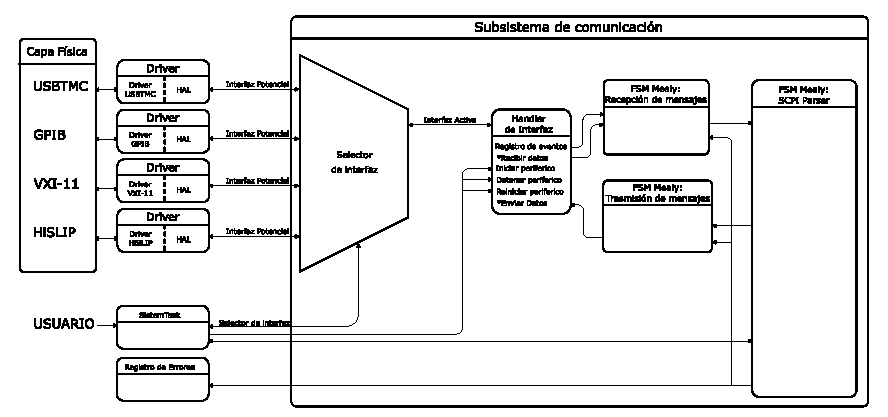
\includegraphics[width=1.0\linewidth]{Figuras/Schems/subsistema-comunicacion_mealy.pdf}
    \caption{Sistema de comunicación con FSMs tipo Mealy.}
    \label{fig:esquema-comunicacion}
\end{figure}

\section{Selector de Medio de Transporte}
\label{sec:selector-transporte}

El subsistema de comunicación opera exclusivamente sobre la interfaz abstracta definida por esta capa y no depende de ninguna implementación particular.

La asociación entre el subsistema de comunicación y una implementación concreta es realizada por un selector de interfaz. Este componente determina cuál de las interfaces disponibles será utilizada por el sistema de acuerdo con la configuración activa del instrumento.

El selector de interfaz no participa en la transferencia ni en el procesamiento de datos. Su única responsabilidad consiste en establecer la asociación entre el subsistema de comunicación y una interfaz de comunicación determinada.

Como consecuencia, el medio de transporte puede modificarse sin requerir cambios en las capas superiores del sistema. Un mismo subsistema de comunicación puede operar sobre USBTMC, GPIB, VXI-11, HiSLIP u otras interfaces compatibles manteniendo inalterada la lógica de procesamiento de comandos y respuestas.

\section{Gestión Interna de Buffers en el Driver}
\label{sec:lock-free-buffers}

Para ofrecer una API de acceso a datos no bloqueante y eficiente a la \textit{Communication Task}, los controladores de la capa física implementan estrategias de sincronización avanzadas que eliminan la necesidad de exclusión mutua tradicional (primitivas de bloqueo) en entornos de tiempo real (RTOS).

\paragraph{Inyección de Dependencias y Propiedad de Memoria}

Para garantizar la independencia absoluta del controlador físico (\textit{driver}), la reserva de memoria para los buffers de comunicación (recepción y transmisión) se realiza en el ámbito de la \textit{Communication Task}. El driver no asigna memoria estática ni dinámica por sí mismo.

Durante la fase de inicialización, la tarea inyecta por referencia estos espacios de memoria (punteros y longitudes) al driver mediante la función \texttt{init()}. Bajo este esquema:
\begin{itemize}
    \item La \textbf{propiedad de la memoria} (\textit{ownership}) reside en la tarea de comunicación, permitiendo ajustar el tamaño de los buffers según los recursos de la plataforma sin modificar la capa física.
    \item El \textbf{control de acceso} se delega al driver, el cual opera directamente sobre esta memoria inyectada. Las rutinas de servicio de interrupción (ISR) o el hardware subyacente escriben los datos y actualizan los índices de escritura (\texttt{head}), manteniendo la estructura conceptual del patrón \textit{lock-free}.
\end{itemize}

\paragraph{Buffer Circular Single-Producer-Single-Consumer (SPSC)}

Para periféricos que disponen de canales de acceso directo a memoria (DMA) o soporte nativo por interrupciones capa a capa (como una UART básica):

\begin{itemize}
    \item La Rutina de Servicio de Interrupción (\textit{ISR}) o el canal DMA actúa como el \textbf{productor} y modifica únicamente el puntero de escritura (\texttt{head}).
    \item La \textit{Communication Task} actúa como el \textbf{consumidor} a través de la función \texttt{get\_char\-\_in()}, modificando únicamente el puntero de lectura (\texttt{tail}).
    \item La detección de desbordamientos (\textit{overflow}) se realiza en el contexto de la ISR comparando la proximidad de ambos punteros, lo que genera de inmediato el evento \texttt{ERR\_BUFFER\_OVERFLOW}.
    \item La tarea procesa los datos de forma segura hasta la posición del \texttt{head} capturada al inicio de su ciclo operativo; las inserciones asíncronas de la ISR no interfieren en la región de memoria leída.
\end{itemize}

\paragraph{Estrategia de Doble Buffer (Even/Odd)}

Para periféricos con restricciones severas de hardware o que carecen de soporte DMA generalizado:
\begin{itemize}
    \item El driver administra dos buffers idénticos en memoria.
    \item La ISR escribe exclusivamente en el buffer definido como activo. Al completarse una transferencia de bloque por hardware, el driver realiza un intercambio de punteros (\textit{swapping}) de forma instantánea.
    \item La \textit{Communication Task} consume los datos del buffer que ha pasado a estar inactivo, mientras el hardware continúa llenando de forma aislada el nuevo buffer activo.
    \item Si al momento de realizar el intercambio por hardware el buffer previo no ha sido procesado por la tarea, el driver bloquea el intercambio y despacha un evento de \texttt{ERR\_BUFFER\_OVERFLOW}.
\end{itemize}

Ambas estrategias mantienen la responsabilidad de detección de errores de transporte/overflow de buffers en la capa de transporte, preservando la independencia.

\section{Mecanismo de Despacho de Eventos y Priorización de Ejecución}
\label{sec:despacho-eventos-prioridad}

Para la sincronización entre el controlador físico (\textit{driver}) y la \textit{Communication Task}, se implementa un registro de eventos centralizado en la interfaz abstracta mediante un mapa de bits (\textit{bitmask}). Debido a que múltiples Máquinas de Estados Finitos (FSM) coexisten secuencialmente dentro del mismo hilo de ejecución, el orden de evaluación de este registro determina la prioridad en la resolución de fallos y el procesamiento de datos.

\subsection{Patrón de Captura Instantánea (\textit{Snapshot}) Atómica}

Para evitar condiciones de carrera entre el contexto de las rutinas de servicio de interrupción (ISR) ---que escriben de forma asíncrona en el registro--- y el contexto de la tarea ---que consume los eventos---, la \textit{Communication Task} no accede de forma directa al mapa de bits del driver durante la ejecución de las FSM. En su lugar, el inicio de cada ciclo operativo de la tarea ejecuta de forma obligatoria el siguiente procedimiento:

\begin{enumerate}
    \item \textbf{Captura Atómica}: Mediante una operación de exclusión mutua elemental (como la inhabilitación temporal de interrupciones o primitivas atómicas del procesador), la tarea lee el registro de eventos del driver y lo copia en una variable local denominada \textit{Snapshot de Eventos}.
    \item \textbf{Limpieza Inmediata}: En la misma sección crítica, el registro de eventos original del driver se borra (o se realiza un \textit{Clear-on-Read}), quedando libre para registrar nuevas notificaciones de la ISR sin interferir con el ciclo actual.
    \item \textbf{Filtrado por FSM}: Cada máquina de estados extrae exclusivamente los bits de su incumbencia desde el \textit{Snapshot de Eventos} local empleando operaciones de enmascaramiento binario (\textit{AND}).
\end{enumerate}

Este enfoque garantiza la coherencia temporal: todas las FSM ejecutan sus transiciones evaluando exactamente el mismo estado del hardware para ese ciclo de reloj del sistema.

\subsection{Orden de Precedencia y Flujo de Control}

El procesamiento de los eventos extraídos del \textit{Snapshot} impone una jerarquía estricta. El bucle de la \textit{Communication Task} evalúa las FSM en un orden decreciente de criticidad, asegurando que cualquier anomalía física severa bloquee el procesamiento de datos inválidos en las capas superiores. El orden de ejecución establecido es el siguiente:

\begin{enumerate}
    \item \textbf{FSM de Gestión de Interfaz (Prioridad Máxima)}: Evalúa en primera instancia los eventos de error crítico del hardware (\texttt{ERR\_HW\_FAIL}) y estados de desconexión. Si se detecta un fallo, esta máquina intercepta el control, ejecuta las rutinas de mitigación o reinicio físico del periférico ((\texttt{reset\_re\-ception()}/\texttt{reset\_trans\-mission()})) y altera el estado global de la interfaz, invalidando los bits de datos del \textit{Snapshot} antes de que pasen a las siguientes etapas.
    \item \textbf{FSM de Recepción (RX)}: Se ejecuta únicamente si la interfaz se encuentra activa y operativa. Extrae los bits correspondientes a la llegada de datos físicos (\texttt{EV\_DATA\_RECEIVED}) o alertas de saturación menores (\texttt{ERR\_BUFFER\_OVERFLOW}). Al procesar los caracteres y validar el delimitador \texttt{LF}, genera el evento lógico interno \texttt{EV\_SCPI\_MSG\_READY}.
    \item \textbf{FSM de Transmisión (TX)}: Procesa los eventos relacionados con el vaciado de buffers físicos o la confirmación de envíos (\texttt{EV\_TX\_COMPLETE}). Su ejecución desacoplada permite liberar recursos de red o puerto serie de forma independiente a la recepción.
    \item \textbf{FSM de Procesamiento SCPI (Prioridad de Aplicación)}: Se ejecuta en la última etapa del ciclo. No consume eventos directos del hardware, sino que reacciona ante los eventos lógicos inyectados por las máquinas de RX y TX en las etapas previas del mismo ciclo, garantizando que el análisis de comandos opere sobre buffers de texto completamente consolidados y validados.
\end{enumerate}

El flujo macroscópico del bucle operativo de la tarea se describe conceptualmente mediante la siguiente secuencia cíclica:

\begin{center}
\small
\texttt{Inicio Bucle} $\rightarrow$ \texttt{Captura Atómica} $\rightarrow$ \texttt{FSM Gestión} $\rightarrow$ \texttt{FSM RX} $\rightarrow$ \texttt{FSM TX} $\rightarrow$ \texttt{FSM SCPI} $\rightarrow$ \texttt{Fin Bucle / Espera}
\end{center}

\subsection{Adaptación al Protocolo SCPI}
\label{subsec:scpi-adaptacion}

Esta sección define cómo la arquitectura segmenta las responsabilidades de procesamiento de datos para la interacción con el motor SCPI.

\paragraph{Detección y Delimitación de Mensajes}

El controlador físico (\textit{driver}) se limita a extraer bytes del medio y notificar su disponibilidad. La delimitación de los mensajes es responsabilidad exclusiva de la máquina de estados de recepción (\textit{RX FSM}) de la \textit{Communication Task}. Esta máquina inspecciona secuencialmente los bytes recuperados mediante la API del driver e identifica el fin de mensaje al detectar el carácter \texttt{LF} (\texttt{0x0A}), en conformidad con la norma IEEE 488.2. Los caracteres \texttt{CR} (\texttt{0x0D}) son ignorados de forma silente durante este proceso de ensamblado.

\paragraph{Separación de Preocupaciones}

\begin{itemize}
    \item \textbf{Mensaje Ensamblado}: Bloque de bytes consolidado en el buffer interno de la \textit{Communication Task}, cuyo término está marcado por el carácter \texttt{LF}.
    \item \textbf{Comando SCPI}: Estructura jerárquica de nodos analizada y parseada, bajo la propiedad exclusiva del motor SCPI.
\end{itemize}

La \textit{Communication Task} entrega la cadena de bytes del mensaje completo al motor SCPI una vez validado el delimitador; el motor SCPI asume de forma independiente las tareas de tokenización, análisis sintáctico y ejecución.

\paragraph{Interrupciones de Consulta (Query Interrupts)}

La capa física no posee noción de interrupciones de consulta. Si el protocolo del periférico subyacente dispone de este mecanismo (por ejemplo, el control de flujo en USBTMC o comandos de desasociación en GPIB), el driver traduce dicha condición de hardware en un evento abstracto de interfaz. La máquina de gestión de la \textit{Communication Task} captura este evento y coordina la acción correspondiente evaluando el estado actual del motor SCPI.

\section{Entorno de Ejecución y Planificación}
\label{sec:entorno-ejecucion}

La \textit{Communication Task} y sus Máquinas de Estados Finitos (FSM) asociadas están diseñadas para operar de manera determinista dentro de un sistema operativo cooperativo secuencial (arquitectura \textit{bare-metal} o \textit{super-loop}). 

Bajo este paradigma, no se requiere la implementación de primitivas de bloqueo complejas (como semáforos o colas de mensajes propias de un RTOS tradicional). Las características del entorno de ejecución son las siguientes:

\begin{itemize}
    \item \textbf{Ejecución No Bloqueante:} Cada FSM evalúa el \textit{Snapshot de Eventos} y retorna inmediatamente el control al planificador si no hay acciones pendientes. El costo computacional (\textit{overhead}) de esta evaluación continua es insignificante.
    \item \textbf{Temporización Simple:} Todo el manejo de tiempos máximos de espera (\textit{timeouts}) para el hardware o la recepción de caracteres incompletos se gestiona mediante una única base de tiempo (\texttt{sys\_tick}) con resolución de 1\,ms.
    \item \textbf{Determinismo:} Al ejecutar todas las fases de comunicación en un único contexto de forma secuencial, se eliminan por diseño las condiciones de carrera y la necesidad de mecanismos de exclusión mutua (\textit{mutexes}) fuera de la captura inicial del \textit{Snapshot}.
\end{itemize}

\section{Integración del Parser SCPI (\texttt{libscpi})}
\label{subsec:integracion-libscpi}

Para el procesamiento sintáctico y semántico de los comandos, la arquitectura contempla la delegación de esta responsabilidad a un motor especializado y conforme al estándar IEEE 488.2, como la biblioteca \texttt{libscpi}. Esta abstracción simplifica la FSM de Procesamiento SCPI, transformándola en una capa de adaptación (\textit{wrapper}) entre los buffers de transporte y el motor lógico.

La integración bidireccional se establece de la siguiente manera:

\paragraph{Flujo de Recepción (RX $\rightarrow$ SCPI)}
Cuando la FSM de Recepción valida la llegada del carácter delimitador (\texttt{LF}) y publica el evento \texttt{EV\_SCPI\_MSG\_READY}, la tarea inyecta el buffer continuo de texto directamente a la biblioteca mediante su API de entrada (ej. \texttt{SCPI\_Input()}). La biblioteca asume internamente el recorrido del árbol de comandos y la ejecución secuencial de los \textit{callbacks} asociados a cada instrumento.

\paragraph{Flujo de Transmisión (SCPI $\rightarrow$ TX)}
Las respuestas generadas por los \textit{callbacks} de la aplicación no acceden directamente al hardware. Se enruta la función de escritura de la biblioteca (ej. el \textit{callback} \texttt{SCPI\_Write()}) para que inserte los datos en el buffer de salida de la tarea y levante el evento lógico \texttt{EV\_SCPI\_TX\_REQ}. En el siguiente ciclo del planificador, la FSM de Transmisión detectará este evento y orquestará el vaciado del buffer hacia el medio físico sin bloquear la ejecución del motor lógico.

\paragraph{Escalabilidad de Contexto}
Aunque el diseño actual ejecuta el motor SCPI de manera cooperativa dentro del mismo bucle de comunicaciones, esta delimitación estricta de interfaces mediante buffers y eventos permite, en futuras iteraciones del proyecto, migrar el procesamiento SCPI a una tarea de menor prioridad independiente, requiriendo únicamente la adición de una cola (\textit{queue}) entre ambas capas lógicas.
